\documentclass[a4paper,10pt,twocolumn]{article}

\usepackage[utf8x]{inputenc}
\usepackage[french]{babel}
\usepackage{graphicx,times}
\usepackage[T1]{fontenc}
\usepackage{amsmath}
\usepackage[font=footnotesize]{caption}
\usepackage{fancyhdr}
\usepackage[explicit]{titlesec}
\usepackage{hyperref}
\usepackage[square,comma,numbers]{natbib}
\usepackage{tabularx}

\newcolumntype{L}[1]{>{\raggedright\arraybackslash}p{#1}}
\newcolumntype{C}[1]{>{\centering\arraybackslash}p{#1}}
\newcolumntype{R}[1]{>{\raggedleft\arraybackslash}p{#1}}

\renewcommand{\bibsection}{}
\def\bibfont{\footnotesize}
\setlength{\bibsep}{0.2em}
\setlength{\bibhang}{10em}

\hypersetup{colorlinks=true, urlcolor=blue, urlbordercolor={0 0 1}, citecolor=black, citebordercolor={1 1 1}}

\addto\captionsfrench{\def\figurename{Fig.}}
\addto\captionsfrench{\def\tablename{Tableau}}

\captionsetup[figure]{labelsep=period, justification=raggedright, singlelinecheck=false}
\captionsetup[table]{labelsep=period, justification=centering, singlelinecheck=false}

\parindent 10pt

\setlength{\voffset}{-1.3in}
\setlength{\topmargin}{1.25cm}
\setlength{\headheight}{1.125cm}
\setlength{\headsep}{0cm}

\setlength{\hoffset}{-1in}
\setlength{\oddsidemargin}{1.3cm}
\setlength{\evensidemargin}{1.3cm}

\setlength{\textheight}{25cm}%23.5
\setlength{\textwidth}{18.5cm}

\setlength{\headsep}{0.67cm}
\setlength{\columnwidth}{8.75cm}
\setlength{\columnsep}{0.63cm}

\setlength{\abovecaptionskip}{0em}
\setlength{\belowcaptionskip}{0em}

\titleformat{\section}
  {\normalfont}{\thesection.}{0.5em}{\MakeUppercase{#1}}
\titleformat{\subsection}
  {\normalfont\itshape}{\thesubsection.}{1.5em}{#1}
\titleformat{\subsubsection}
  {\normalfont\itshape}{\thesubsubsection.}{1.5em}{#1}
	
\titlespacing\section{0pt}{1em}{0.5em}
\titlespacing\subsection{0pt}{1em}{0.5em}
\titlespacing\subsubsection{0pt}{1em}{0.5em}

\fancyhf{}
\fancyhead[R]{\fontsize{8pt}{8pt}\selectfont \textbf{S}YMPOSIUM DE \textbf{G}ENIE \textbf{E}LECTRIQUE (SGE 2018), 3-5 JUILLET 2018, NANCY, FRANCE}
\renewcommand{\headrulewidth}{0pt}


\pagestyle{empty}


\title{
\fontsize{24pt}{24pt}\selectfont
Titre de la communication (Style ‘Titre’)
}

\author{
\fontsize{11pt}{11pt}\selectfont
Prénom NOM des auteurs (Style ‘Nom’)\\
\fontsize{10pt}{10pt}\selectfont
Affiliation des auteurs (Style ‘Affiliation’)
}

\date{}


\begin{document}

\maketitle
\thispagestyle{fancy}


\fontsize{9pt}{9pt}\selectfont
\textbf{RESUME -- Écrire un résumé de la communication de 15 lignes maximum. Ce résumé doit présenter de façon synthétique les objectifs du travail présenté, les principaux résultats et insister sur les originalités du travail. (Style ‘Résumé’)}\\

\textbf{\textit{Mots-clés -- Écrire ici une liste n’excédant pas 8 mots-clés significatifs. (Style ‘Mots-Clés’).}}

\fontsize{10pt}{10pt}\selectfont


\section{Introduction  (Style ‘Titre 1’)}

Décrire le contexte et les objectifs du travail. Positionner le travail par rapport à la littérature et aux principaux travaux antérieurs. Présenter le plan de la communication. (Style ‘Normal’).


\section{Titre de section (Style ‘Titre 1’)}

Développer dans les sections, sous-sections et sous sous-sections (ne pas excéder 3 niveaux hiérarchiques) les travaux réalisés en présentant les grandes étapes et les principaux résultats.

\textbf{Le résumé final de la communication doit comporter au maximum 2 pages et doit respecter le format décrit dans ce document. La taille du fichier pdf est par ailleurs limitée à 3.5 Mo.}


\subsection{Titre de sous-section (Style ‘Titre 2’)}

Les tableaux, figures et équations doivent respecter les numérotations et formats ci-après. Les figures (Style ‘Images’) et tableaux (Style ‘Tableaux’) doivent être centrés et légendées. Les équations (Style ‘Equation’, 10 pts, centré) seront centrées et numérotées (style ‘Numéro d’équation’, Times New Roman, 10 pts, aligné à droite) et une ligne pourra être laissée libre avant et après chaque équation.

\begin{figure}[!ht]
	\begin{center}
		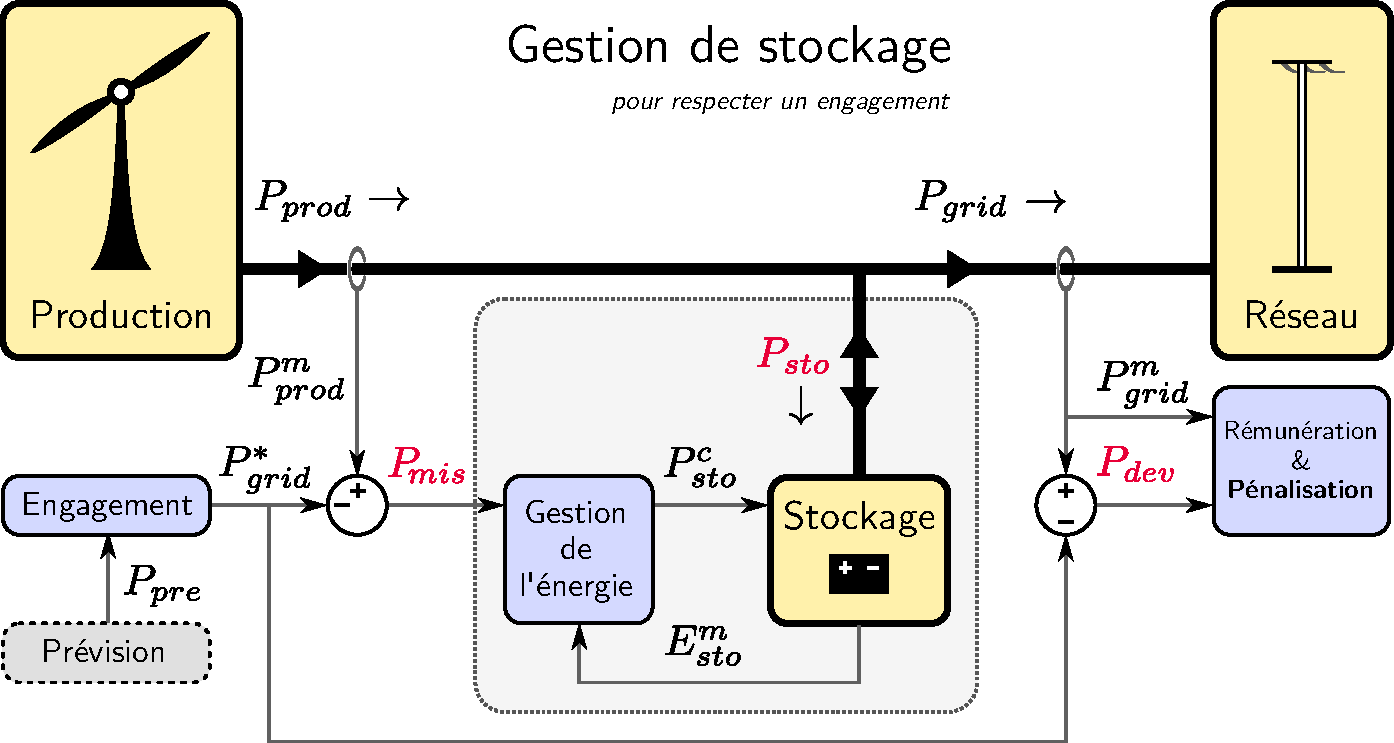
\includegraphics[width=0.6\columnwidth]{figures/wind_storage.pdf}
	\end{center}
	
	\caption{Titre de la figure (Style ‘Légende’)}
	\label{fig_1}
\end{figure}

\begin{table}[!h]
	\caption{Mettre ici le titre du tableau}
	
	\begin{center}
		\begin{tabular}{|>{\footnotesize}L{1.4cm}|>{\footnotesize}L{1.5cm}|>{\footnotesize}L{2.4cm}|>{\footnotesize}L{2.1cm}|}
			\hline
			\textbf{Titre colonne 1} & \textbf{Titre colonne 2} & \textbf{Style (‘Titre colonnes tableaux’)} & \textbf{} \\
			\hline
			Donnée 1 & Style (Cellules tableaux’) & & \\
			\hline
			Donnée 2 & & & \\
			\hline
		\end{tabular}
	\end{center}
	
	\label{tab_1}
\end{table}

\subsubsection{Titre de sous sous-section (Style ‘Titre 3’)}

\begin{equation}
	y = f(x) + \sum_{k=1}^{\infty} h_k \cdot sin(k \omega t)
	\label{eq_1}
\end{equation}


\section{Soumission de la communication}

La soumission se fait en ligne à partir du site électronique de la conférence : \url{http://sge2018.sciencesconf.org} (voir la rubrique ‘Soumission en ligne des communications’).\\

Le fichier soumis sera préalablement converti au format PDF avec les polices incorporées et ne devra pas excéder la taille maximale de 3.5 Mo.


\section{Conclusions}

Rappeler les principaux résultats marquants et originaux du travail. Le cas échéant, proposer des perspectives au travail présenté.


\section{Remerciements}

Cette partie (facultative) doit être placée entre la conclusion et les références.


\section{Références}

Citer ici les principales références du travail réalisé (style ‘Références’). Privilégier les références les plus pertinentes et les publications originelles. Numéroter les références de la même façon que dans l’exemple ci-dessous – par ordre d’apparition dans le texte.


\begin{thebibliography}{1}

\bibitem{bib_1}{T. Lubin, K. Berger, et A. Rezzoug, « Inductance and Force Calculation for Axisymmetric Coil Systems Including an Iron Core of Finite Length », Progress In Electromagnetics Research B, vol. 41, p. 377 396, juin 2012.}

\bibitem{bib_2}{A. Wiederhold et al., « Electric and Magnetic Characterization of Bulk Ag-added MgB2 », in Superconductivity: Applications Today and Tomorrow, J. Muralidhar Miryala (Shibaura Institute of Technology Toyosu, Koto-ku, Tokyo, Éd. Nova Science Publishers, 2015, Chapter 12, p. 269 277.}

\bibitem{bib_3}{K. Berger et al., « Benchmark on the 3D Numerical Modeling of a Superconducting Bulk », in 21st International Conference on the Computation of Electromagnetic Fields (Compumag 2017), Daejeon, South Korea, 2017, (ID 110).}

\end{thebibliography}


\end{document}

